%\subsection{Metodologia badawcza}\label{subsec:metodologia-badawcza}
Najbardziej oczywistą, a zarazem najłatwiejszą do wykonania metodą porównawczą było rozegranie określonej liczby pojedynków pomiędzy oponentami, a następnie sprawdzenie współczynnika wygranych.
Do przeprowadzenia testów wykorzystano program komputerowy Cutechess \cite*{cutechess}.
Posłużył on nie tylko jako szachowy interfejs graficzny, ale także jako zarządca turniejowy dla silników implementujących protokół UCI.

Pomiędzy wybranymi parami silników rozegrano po 25 gier, każda trwająca $1$ minutę na~partię plus $0,6$~sekundy na ruch.
Aby zmniejszyć powtarzalność, gry rozpoczynały się~nie~od~pozycji startowej, ale od losowych otwarć szachowych z biblioteki \cite{lichess-book}.
Pozycje te~były wyrównane, aby~uniknąć przewagi początkowej któregokolwiek z silników.


\subsection{Wybrane wyniki}\label{subsec:wybrane-wyniki}

\subsubsection{Tablica figur}
\begin{figure}[ht]
    \centering
    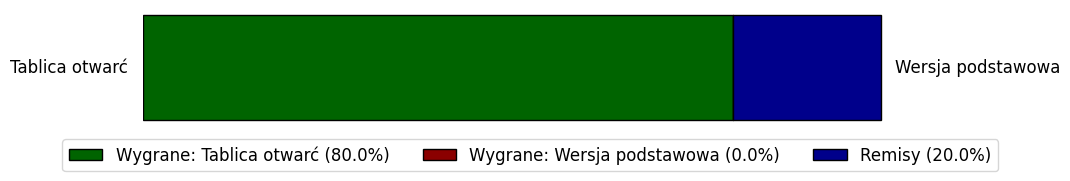
\includegraphics[width=1\linewidth]{rozdzialy/rozdzial03/1_porownanie-wersji-silnika/rysunki/wyniki-tablica}
    \caption{Wyniki rozgrywek z tablicą figur}
    \label{fig:wyniki-tablica}
\end{figure}
Silnik z zaimplementowaną tablicą figur uzyskał znaczną przewagę nad swoim rywalem.
Nie tylko nie przegrał ani jednej partii, ale wygrał aż 80\% z nich.
Świadczy to o zwiększeniu dokładności oceny heurystycznej pozycji, co przełożyło się na możliwość podejmowania lepszych decyzji w trakcie gry.


\subsubsection{Struktura pionów i bezpieczeństwo króla}
\begin{figure}[ht]
    \centering
    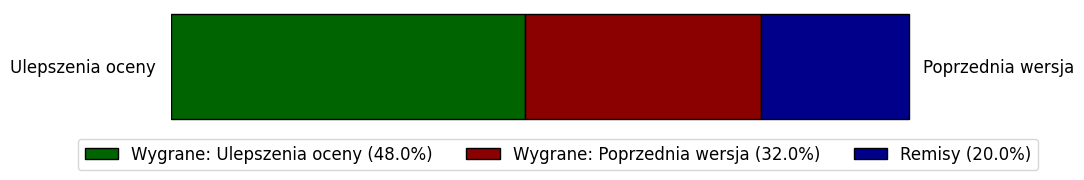
\includegraphics[width=1\linewidth]{rozdzialy/rozdzial03/1_porownanie-wersji-silnika/rysunki/wyniki-full-eval}
    \caption{Wyniki rozgrywek ze strukturą pionów i bezpieczeństwem króla}
    \label{fig:wyniki-full-eval}
\end{figure}
Poprzednią wersję implementującą tablicę figur porównano z wersją, która dodatkowo posiadała ulepszenia w postaci struktury pionów oraz oceny bezpieczeństwa króla.
Wyniki były bardziej zbliżone niż w poprzednim pojedynku, co sugeruje ich mniejszy wpływ na siłę silnika.
Niemniej, były one na tyle znaczące, aby zagwarantować wygraną na poziomie 48\%.
Z analizy pojedynczych partii wynikało, że silnik z ulepszeniami zyskiwał przewagę już w pierwszych ruchach gry, co  pozwalało mu na kontrolę nad planszą w późniejszych etapach.


\subsubsection{Alfa-Beta cięcie}
\begin{figure}[ht]
    \centering
    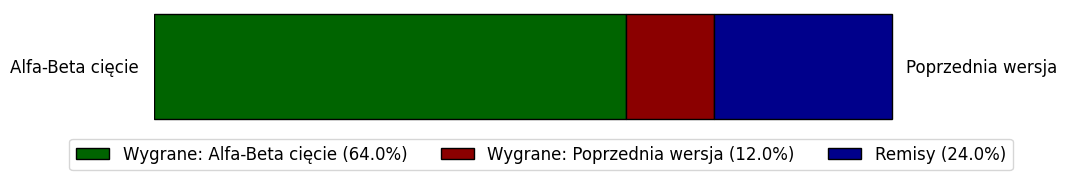
\includegraphics[width=1\linewidth]{rozdzialy/rozdzial03/1_porownanie-wersji-silnika/rysunki/wyniki-alfa-beta}
    \caption{Wyniki rozgrywek z alfa beta cięciem}
    \label{fig:wyniki-alfa-beta}
\end{figure}
Pierwsze sprawdzone ulepszenie co do algorytmów przeszukiwania drzewa gry przyniosło oczekiwane rezultaty.
Zmniejszenie liczby odwiedzonych węzłów pozwoliło na zwiększenie głębokości przeszukiwań, a co za tym idzie, pozwoliło silnikowi na lepsze ocenianie pozycji.
Wynik 64\% wygranych oraz 24\% remisów utwierdza w przekonaniu o poprawności i~skuteczności implementacji algorytmu alfa-beta.


\subsubsection{Ewaluacja stanów cichych}
\begin{figure}[ht]
    \centering
    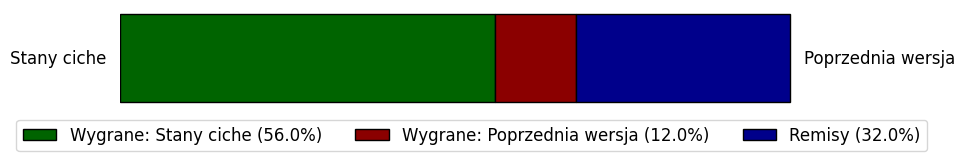
\includegraphics[width=1\linewidth]{rozdzialy/rozdzial03/1_porownanie-wersji-silnika/rysunki/wyniki-stany-ciche}
    \caption{Wyniki rozgrywek z ewaluacją stanów cichych}
    \label{fig:wyniki-stany-ciche}
\end{figure}
Wykonanie testów dla tego ulepszenia było szczególne istotne, z tego względu, że dodatkowa ewaluacja stanów cichych ma także tendencje do zwiększenia liczby odwiedzonych węzłów drzewa.
Należało potwierdzić, że zysk związany z uniknięciem efektu horyzontu przewyższa koszty związane z dodatkowymi obliczeniami.
Jak widać na rysunku \ref{fig:wyniki-stany-ciche}, silnik z ulepszeniem wygrał 56\% i zremisował 32\% partii, co sugeruje, że dodatkowe obliczenia były warte podjęcia.

\subsubsection{Statyczne sortowanie ruchów}

\begin{figure}[ht]
    \centering
    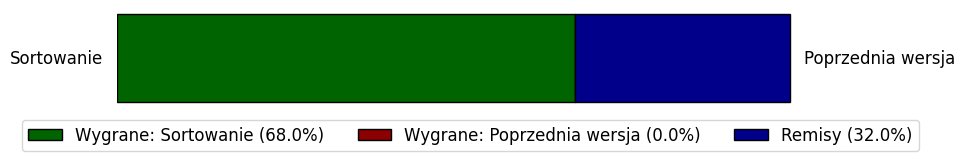
\includegraphics[width=1\linewidth]{rozdzialy/rozdzial03/1_porownanie-wersji-silnika/rysunki/wyniki-sortowanie}
    \caption{Wyniki rozgrywek ze statycznym sortowaniem ruchów}
    \label{fig:wyniki-sortowanie}
\end{figure}
Wyniki pojedynku pomiędzy poprzednią wersją silnika a wersją z zaimplementowanym statycznym sortowaniem ruchów były zaskakująco korzystne.
Silnik z ulepszeniem wygrał 68\% partii, przy jednoczesnym braku jakiejkolwiek porażki.
Jeszcze raz potwierdza to znaczenie ułożenia odwiedzanych wierzchołków dla algorytmu alfa-beta.

\subsubsection{Tabela transpozycji}
\begin{figure}[ht]
    \centering
    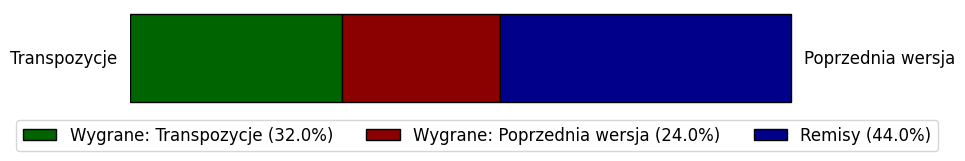
\includegraphics[width=1\linewidth]{rozdzialy/rozdzial03/1_porownanie-wersji-silnika/rysunki/wyniki-transpozycje}
    \caption{Wyniki rozgrywek z tabelą transpozycji}
    \label{fig:wyniki-transpozycje}
\end{figure}
Otrzymane rezultaty dla ulepszenia związanego z tabelą transpozycji wskazywały na~niedokładność w implementacji.
Nowy silnik remisował większość pojedynków.
Analiza poszczególnych rozgrywek wskazywała, że silnik z ulepszeniem w~większości zremisowanych gier obejmował zauważalne prowadzenie.
Jednym z~możliwych powodów mogło być~nierozróżnianie oceny jednej pozycji planszy, od~drugiej, takiej samej, ale~prowadzącej do~niekorzystnego remisu (np. trzykrotne powtórzenie).
W efekcie silnik zapętlał się w pozycji z jego perspektywy korzystnej, prowadząc do remisu.
Poprawa implementacji polegałaby na~stworzeniu oddzielnego haszowania rozróżniającego te dwie, na pozór identyczne, pozycje.
Innym rozwiązaniem byłoby sprawdzenie, czy nastąpił remis, przed zwróceniem wartości z~tabeli transpozycji.


\subsection{Podsumowanie}\label{subsec:podsumowanie}
Powyżej przedstawiono te z wyników, które miały największy wpływ na siłę silnika, bądź przedstawiały ciekawe zależności.
Biblioteka otwarć, choć istotna, nie została porównana, gdyż rozgrywki rozpoczynały się od wyrównanych pozycji w grze środkowej.

W pozostałych ulepszeniach wynik był znacznie bardziej wyrównany, zahaczający o~błąd statystyczny.
Aby przeprowadzić analizę tych usprawnień, należałoby przeprowadzić więcej rozgrywek pomiędzy silnikami, bądź skorzystać z bardziej wyrafinowanych metod statystycznych.
Jedną z takich technik, powszechnie stosowanych w silnikach szachowych, jest Sekwencyjny Test Probabilistyczny (ang. \emph{Sequential Probability Ratio Test}, SPRT).
Pozwala on na zwiększenie wiarygodności wyników, przy jednoczesnym zredukowaniu do minimum liczby przeprowadzanych rozgrywek \cite*{wiki-sprt}.
Choć program Cutechess posiada również możliwość przeprowadzenia SPRT, wykraczały one poza zakres niniejszej pracy.


%Największe różnice zaobserwowano w ulepszeniach:
%\begin{itemize}
%    \item \textbf{Tablica figur} – współczynnik wygranej dla tego ulepszenia sięgnął 90\%.
%    Wynikło to po części z tego, że silnik uzyskał o wiele więcej informacji co do pozycjonowania konkretnych figur na planszy.
%    Z drugiej strony mogło to wynikać z przewidywalności ruchów z uwagi na determinizm silnika.
%    Po zaimplementowaniu tablicy otwarć gry były bardziej losowe.
%    \item \textbf{Sortowanie ruchów} – lorem ipsum dolor sit amet, consectetur adipiscing elit.
%\end{itemize}
%
%%\subsection{Najmniej istotne ulepszenia}
%Najmniejsze różnice zaobserwowano natomiast w ulepszaniach:
%\begin{itemize}
%    \item \textbf{Ochrona króla} – wersja ulepszona, jak i poprzednia otrzymały po 50\% wygranych.
%    Przypuszczeniem autora jest, że zmianńoa heurystyki dotyczyła bardzo specyficznych sytuacji, które nie miały dużego wpływu na ogół rozgrywek.
%    \item \textbf{Biblioteka otwarć} – nie porównano wersji z biblioteką otwarć, gdyż rozgrywki rozpoczynają się od wyrównanych pozycji w grze środkowej, a więc biblioteka otwarć nie miałaby wpływu na wynik.
%\end{itemize}
%
%\begin{figure}[ht]
%    \centering
%    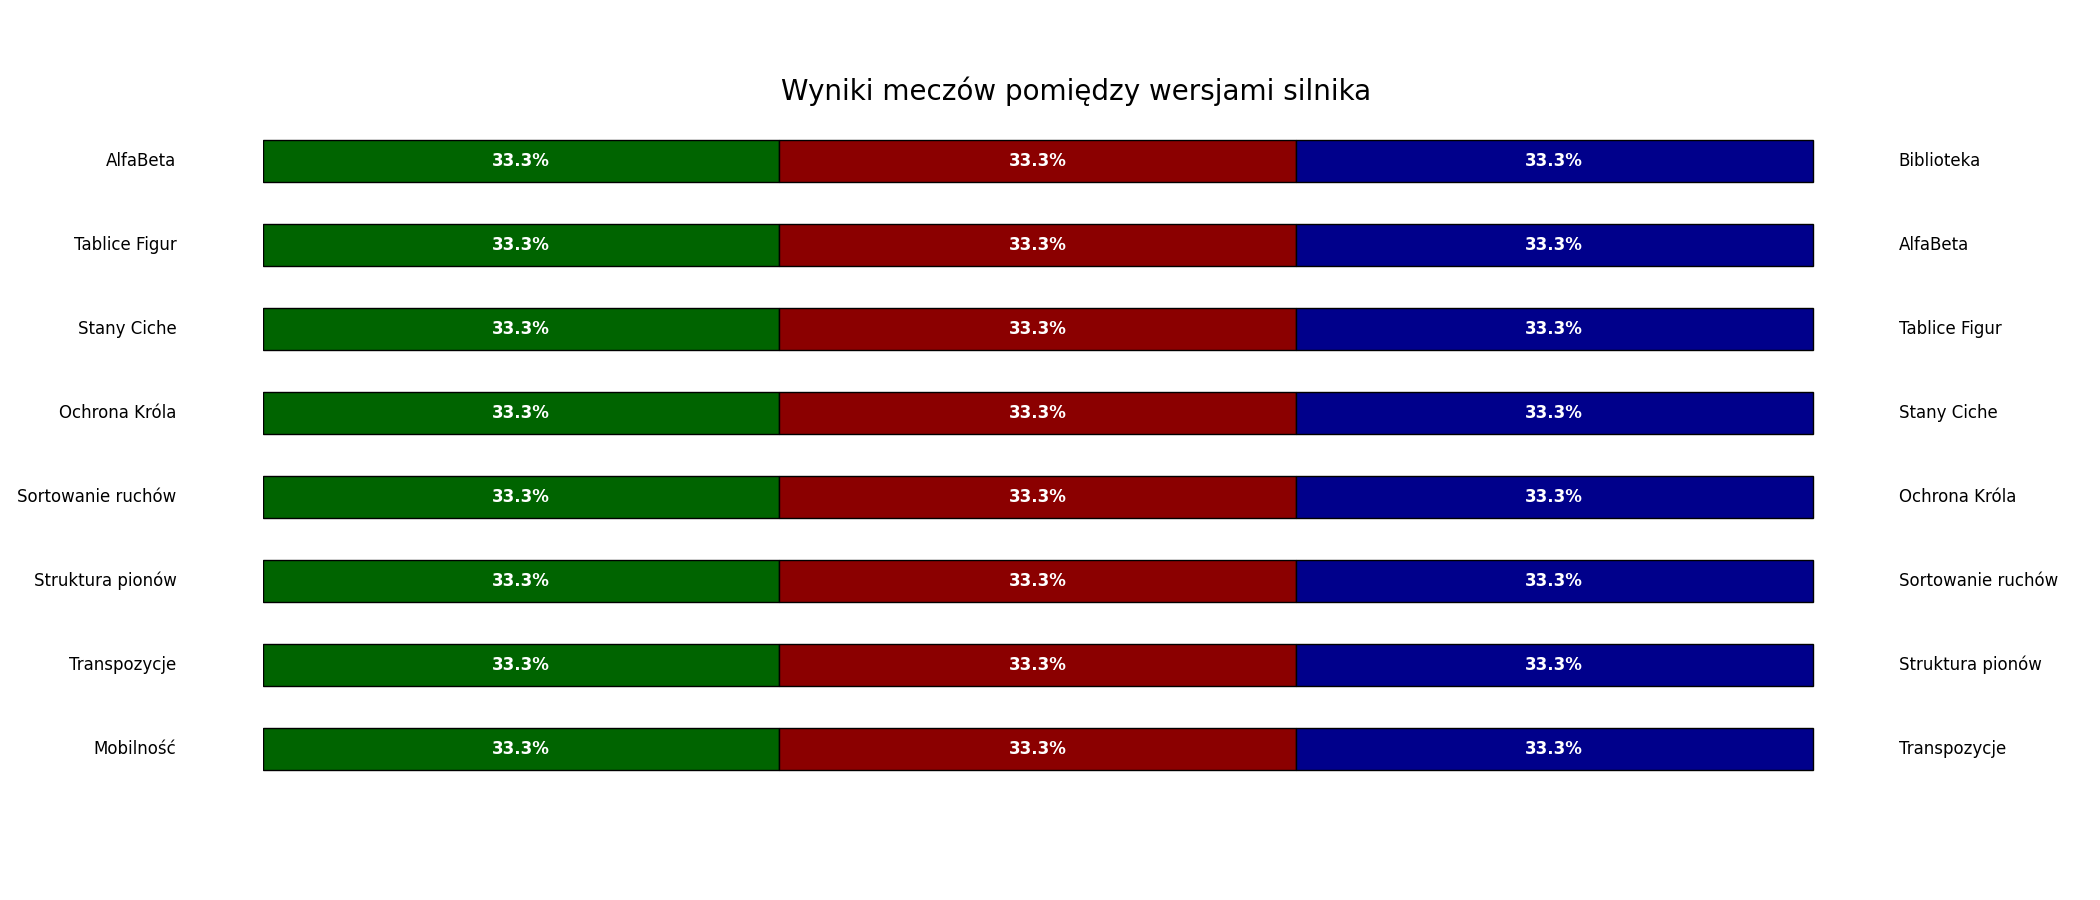
\includegraphics[width=1\linewidth]{rozdzialy/rozdzial03/1_porownanie-wersji-silnika/rysunki/gry-wyniki}
%    \caption{Wyniki rozgrywek pomiędzy wersjami silnika}
%    \label{fig:wyniki-wersje}
%\end{figure}